\documentclass[../CMPUT-404-Notes.tex]{subfiles}
\begin{document}
The internet is made up with multiple layers of protocols and mediums that allows communications between computers.
\section{Link Layer}
\begin{quotebox}
  In computer networking, the link layer is the lowest layer in the Internet protocol suite, the networking architecture of the Internet. The link layer is the group of methods and communications protocols confined to the link that a host is physically connected to. The link is the physical and logical network component used to interconnect hosts or nodes in the network and a link protocol is a suite of methods and standards that operate only between adjacent network nodes of a network segment.

  From: https://en.wikipedia.org/wiki/Link\_layer
\end{quotebox}
\subsection{Ethernet}
On a wired connection all information will need to be cut up into an \emph{Ethernet} frame.\\

\subsubsection{Ethernet Header Sizes}
{\centering
\begin{DndTable}[color=PhbLightGreen]{XX}
  \textbf{Schema} & \textbf{Size in bytes} \\
  Preamble & 7 \\
  Start Frame Delimiter & 1 \\
  Destination & 6 \\
  Source & 6 \\
  Length & 2 \\
  Payload & 46-1500 \\
  CRC & 4 \\
\end{DndTable}}

The preamble will always be 0xAA because 0xAA is encoded as 10101010 in 8-bit binary. This will set the sample rate for the hardware to listen, spool up and grab the information.
The Start Frame Delimiter or SFD denotes the start of the Ethernet frame, it is encoded as 0xAB or 10101011, the double 1 at the end will tell the hardware to process the next 64-1518 bytes. 
The \textbf{Source} and \textbf{Destination} sections are MAC addresses that are mapped to hardware and tells who is the recipient and sender. 
\textbf{Length} is the size of the payload in byte units. \textbf{Payload} contains the actual data itself. The standard assumes a MTU or Maximum Transfer Unit of 1500 bytes, and the \textbf{CRC} is used as a checksum and error detection.

\begin{Note}
  This is a pretty old standard and in today's world we might use something faster or bigger in terms of payload size.  
\end{Note}

The standard is designed so that everyone knows the minimum packet size that can be sent. 
Note that there are potential wastes in a transmission.
Also note that sizes that aren't fragmented or split will lead to minimal latency from the lack of overhead caused by splitting packets.

The idea is to keep the message sizes smaller than 1.5kb to ensure that you stay inside within packets, but not too small so that you send too many headers. Most people have MTUs at 1500 or less.


\section{Internet Layer}
\begin{quotebox}
  The internet layer is a group of internetworking methods, protocols, and specifications in the Internet protocol suite that are used to transport network packets from the originating host across network boundaries; if necessary, to the destination host specified by an IP address. The internet layer derives its name from its function facilitating internetworking, which is the concept of connecting multiple networks with each other through gateways.

  From: https://en.wikipedia.org/wiki/Internet\_layer
\end{quotebox}
\subsection{IPV4}
This is a routing standard that allows the Ethernet frame/data to be routed. This is because Ethernet is not routable. 
IPV4 is the backboard of the internet but we are running out of IPV4 addresses. 
It was designed to communicate over large distances and to many computers, in fact it was a compromise to address computers instead of using MAC addresses. 
Note IPV4 is stateless as well.
The IPV4 header is wrapped into the Ethernet Frame.

\begin{figure}[!h]
  \centering
  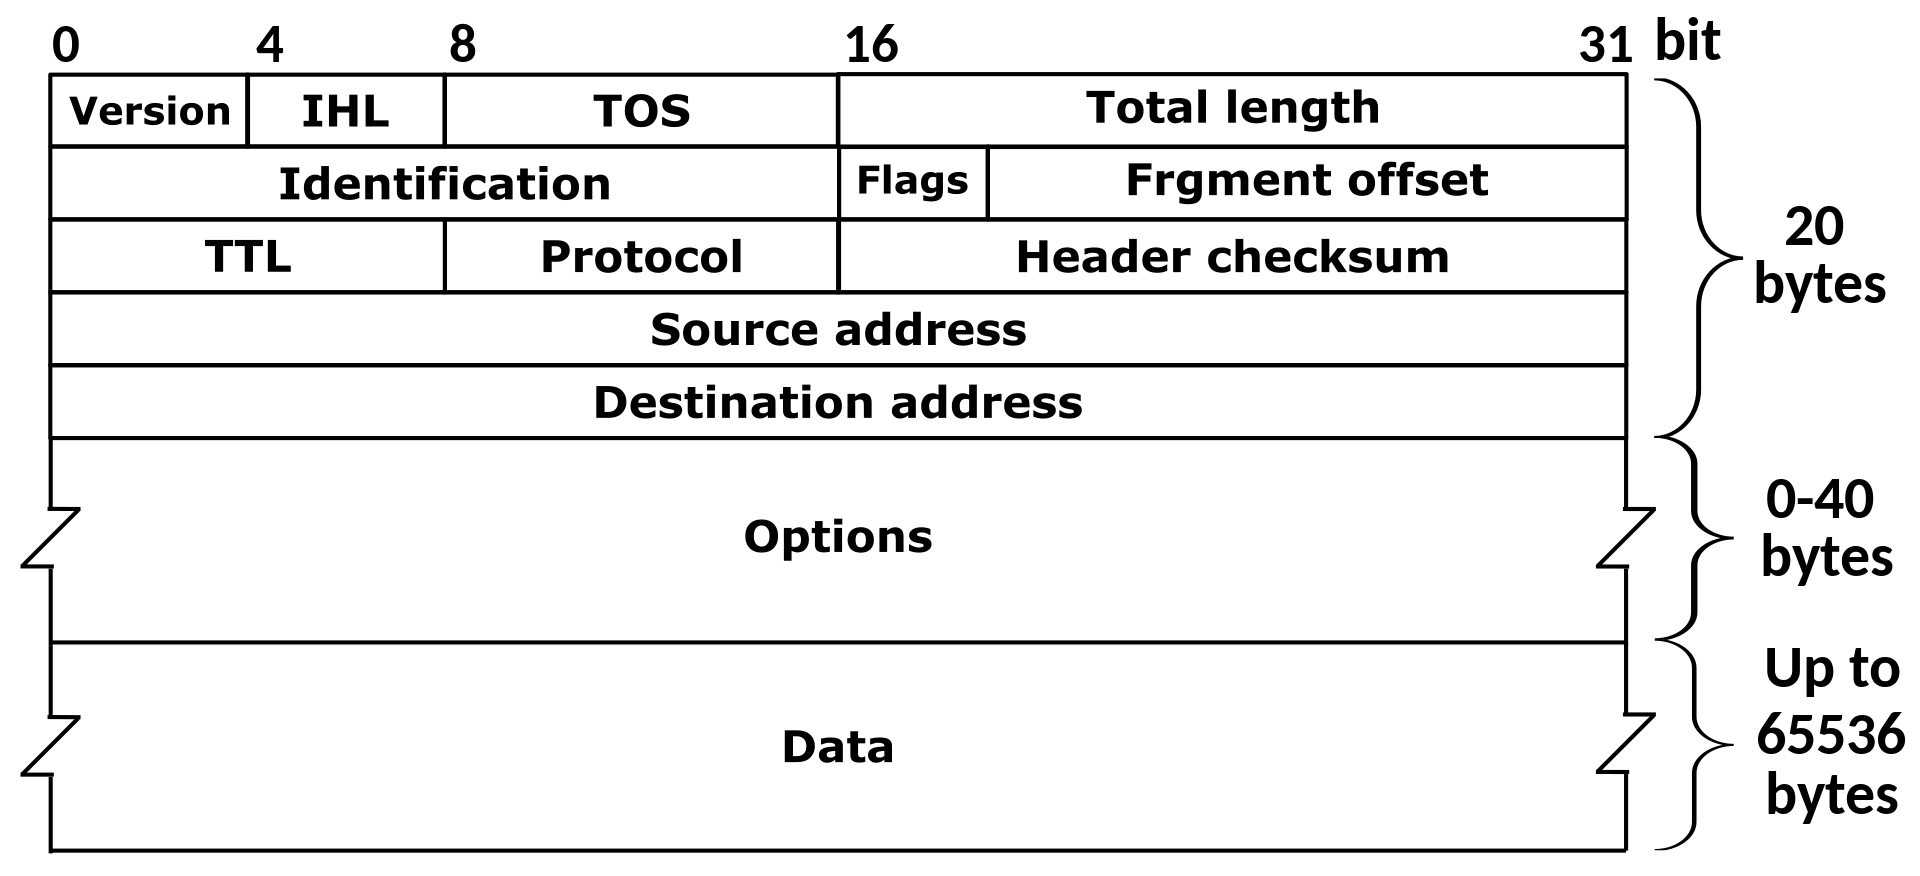
\includegraphics[width=\columnwidth]{../assets/IPv4-Packet-en.png}
  \caption{IPV4 header}
  \label{fig:-assets-IPv4-Packet-en-svg-png}
  https://en.wikipedia.org/wiki/IPv4\#/media/File:IPv4\_Packet-en.svg
\end{figure}

\subsection{IPV6}
IPV6 is like IPV4 but with more addresses. The number of addresses you can represent using IPV6 is $2^{128}$ while IPV4 can only represent around 4.2 billion values $2^{32}$. 
TCP is encapsulated within the IPV6 layer.  
An address can be really big, Examples
\begin{itemize}
  \item 2001:0bd8:0000:0000:0000:0000:0000:00001
  \item 3132:0:0:0:0:0:0:1
  \item 2001:bd8::1
\end{itemize}
For ports the IPV6 addresses are encompassed within square brackets. Example: http://[2001:29b::1]:443/

\begin{figure}[!h]
  \centering
  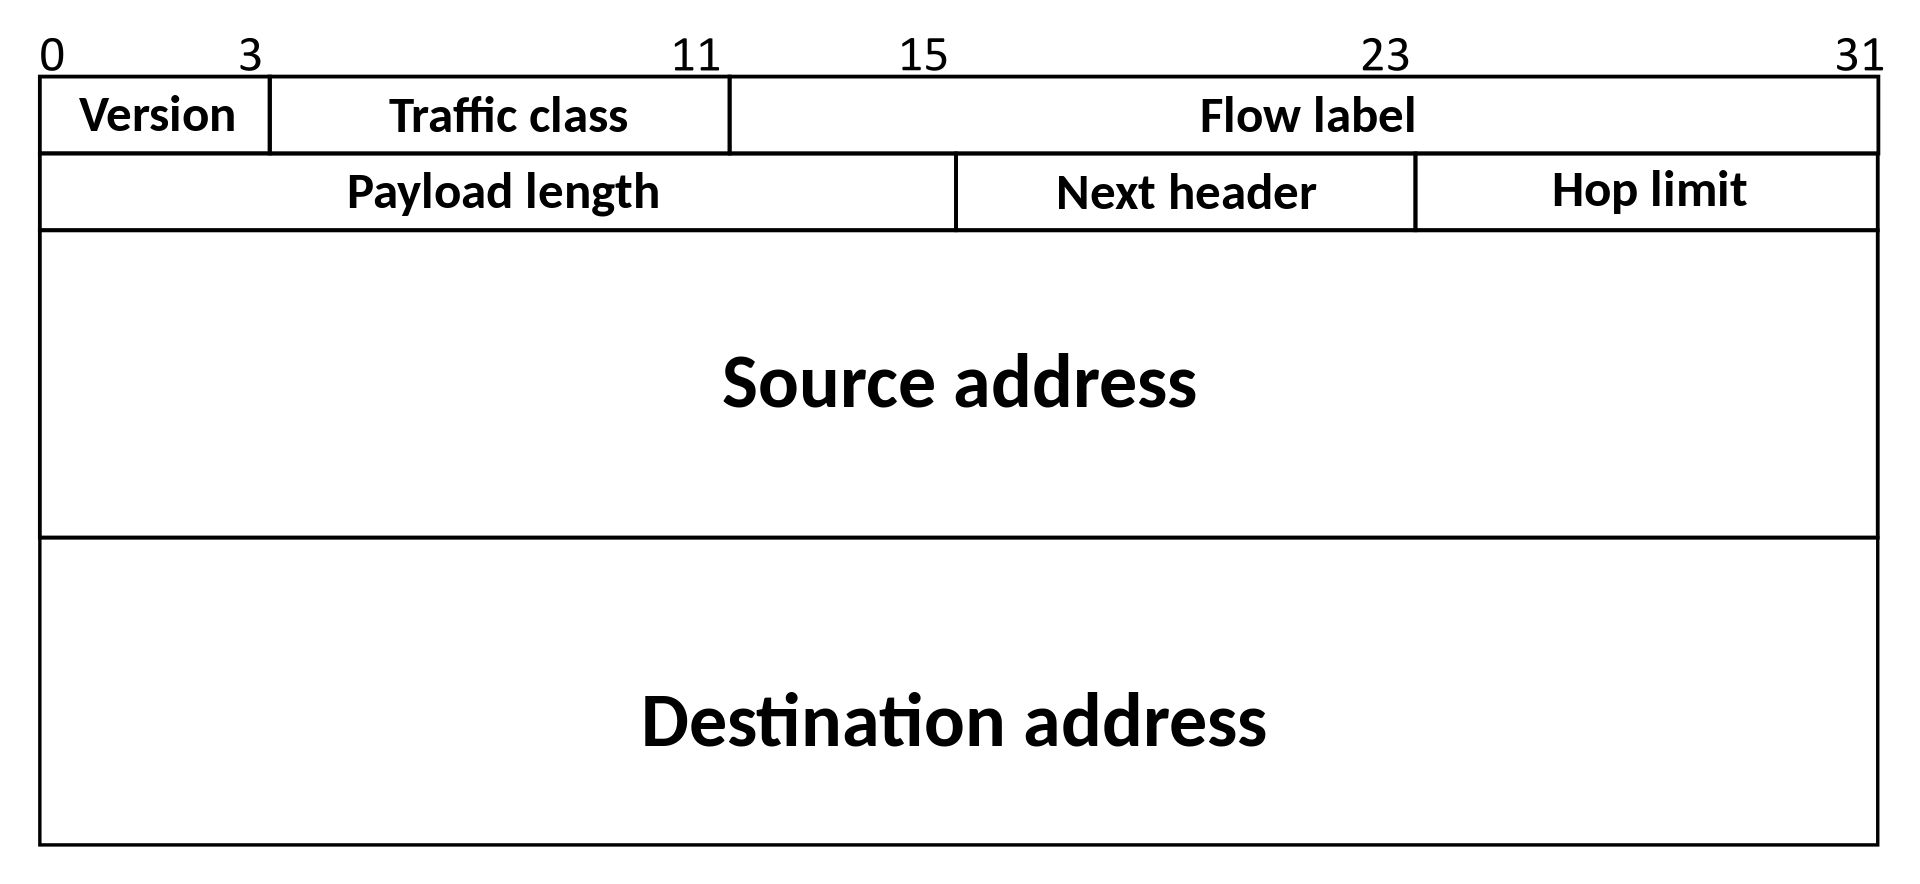
\includegraphics[width=\columnwidth]{../assets/IPv6-header-en.png}
  \caption{IPV6 Header}
  % \label{fig:-assets-IPv6_header-en-svg-png}
  https://en.wikipedia.org/wiki/IPv6\#/media/File:IPv6\_header-en.svg
\end{figure}

\begin{Note}
  The IPV6 header is much simpler compared to the IPV4 header as the designers of the IPV6 header wanted to keep the header simple and have a different protocol handle everything else. For integrity protection that task is handled by the link layer e.g., Ethernet, and the transport layer, mainly TCP or UDP. 
\end{Note}

\section{Transport Layer}
\begin{quotebox}
  In computer networking, the transport layer is a conceptual division of methods in the layered architecture of protocols in the network stack in the Internet protocol suite and the OSI model. The protocols of this layer provide host-to-host communication services for applications. It provides services such as connection-oriented communication, reliability, flow control, and multiplexing.

  From: https://en.wikipedia.org/wiki/Transport\_layer
\end{quotebox}
\subsection{UDP}
Stands for \textbf{User Datagram Protocol}, the user means that user-space applications can use it. Like IPV4 it's stateless, and only contains source and destination port numbers as well as a checksum to provide some integrity. 
This type of connection is lossy and not ordered, meaning deterministic behavior is not guaranteed. 
There is also no connections like TCP.
This is useful for only sending a small amount of data across a network where latency is more important than integrity.
UDP is encompassed within IP, the data comes after it. It will be the IP data size minus the UDP header size.
Checksum is not required but includes data, UDP header and IP header. 
DNS or NTP uses UDP because they are simple query-responses that can fit within a UDP message packet, of \(2^{16} = 65536\) bytes.

\begin{figure}[!h]
  \centering
  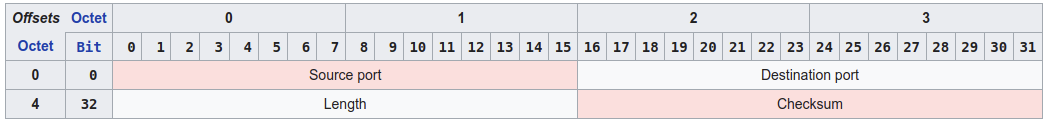
\includegraphics[width=\columnwidth]{../assets/UDP-header.png}
  \caption{UDP Header}
  % \label{fig:-assets-UDP-header-png}
  https://en.wikipedia.org/wiki/User\_Datagram\_Protocol
\end{figure}

\subsection{TCP}
Stands for Transmission Control Protocol. Unlike UDP there is a connection between a socket that goes through different states. 
Some of these states are part of the 3-packet handshake that an opening connection makes before sending data. 
This 3-packet handshake involves 
\begin{enumerate}
  \item The source socket will send a SYN to the destination socket who is listening
  \item That destination socket will reply with SYN+ACK to tell the incoming connection "I've heard you SYN"
  \item Finally the source socket will reply the destination socket's SYN+ACK with ACK to say "I've heard your SYN+ACK let's communicate"
\end{enumerate}

There are two ways a TCP connection can close:
\subsubsection{Active Close}
This is initiated by the client and will send a CLOSE/FIN signal to the server, the server will respond with ACK in which the client will respond with FIN/ACK.
The client could also close the connection and send the FIN+ACK/ACK at the same time to the server and ignore the response from the server.

\subsubsection{Passive Close}
In passive close the server will disconnect the connection with a FIN/ACK, and have the client respond with CLOSE/FIN with the server responding with ACK after CLOSE/FIN.

\begin{figure}[!h]
  \centering
  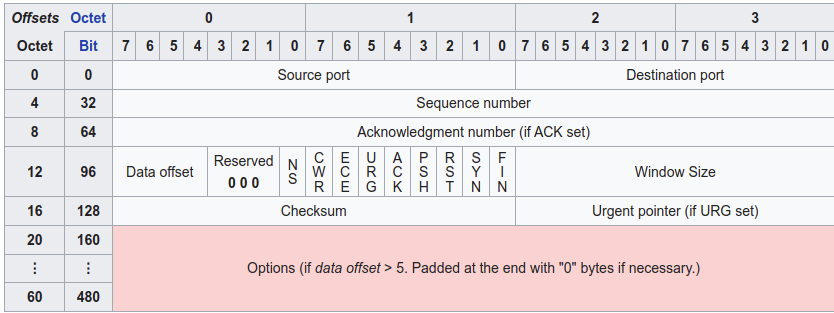
\includegraphics[width=\columnwidth]{../assets/TCP-header.png}
  \caption{TCP Header}
  % \label{fig:-assets-TCP-header-png}
  https://en.wikipedia.org/wiki/Transmission\_Control\_Protocol
\end{figure}

\begin{figure}[!h]
  \centering
  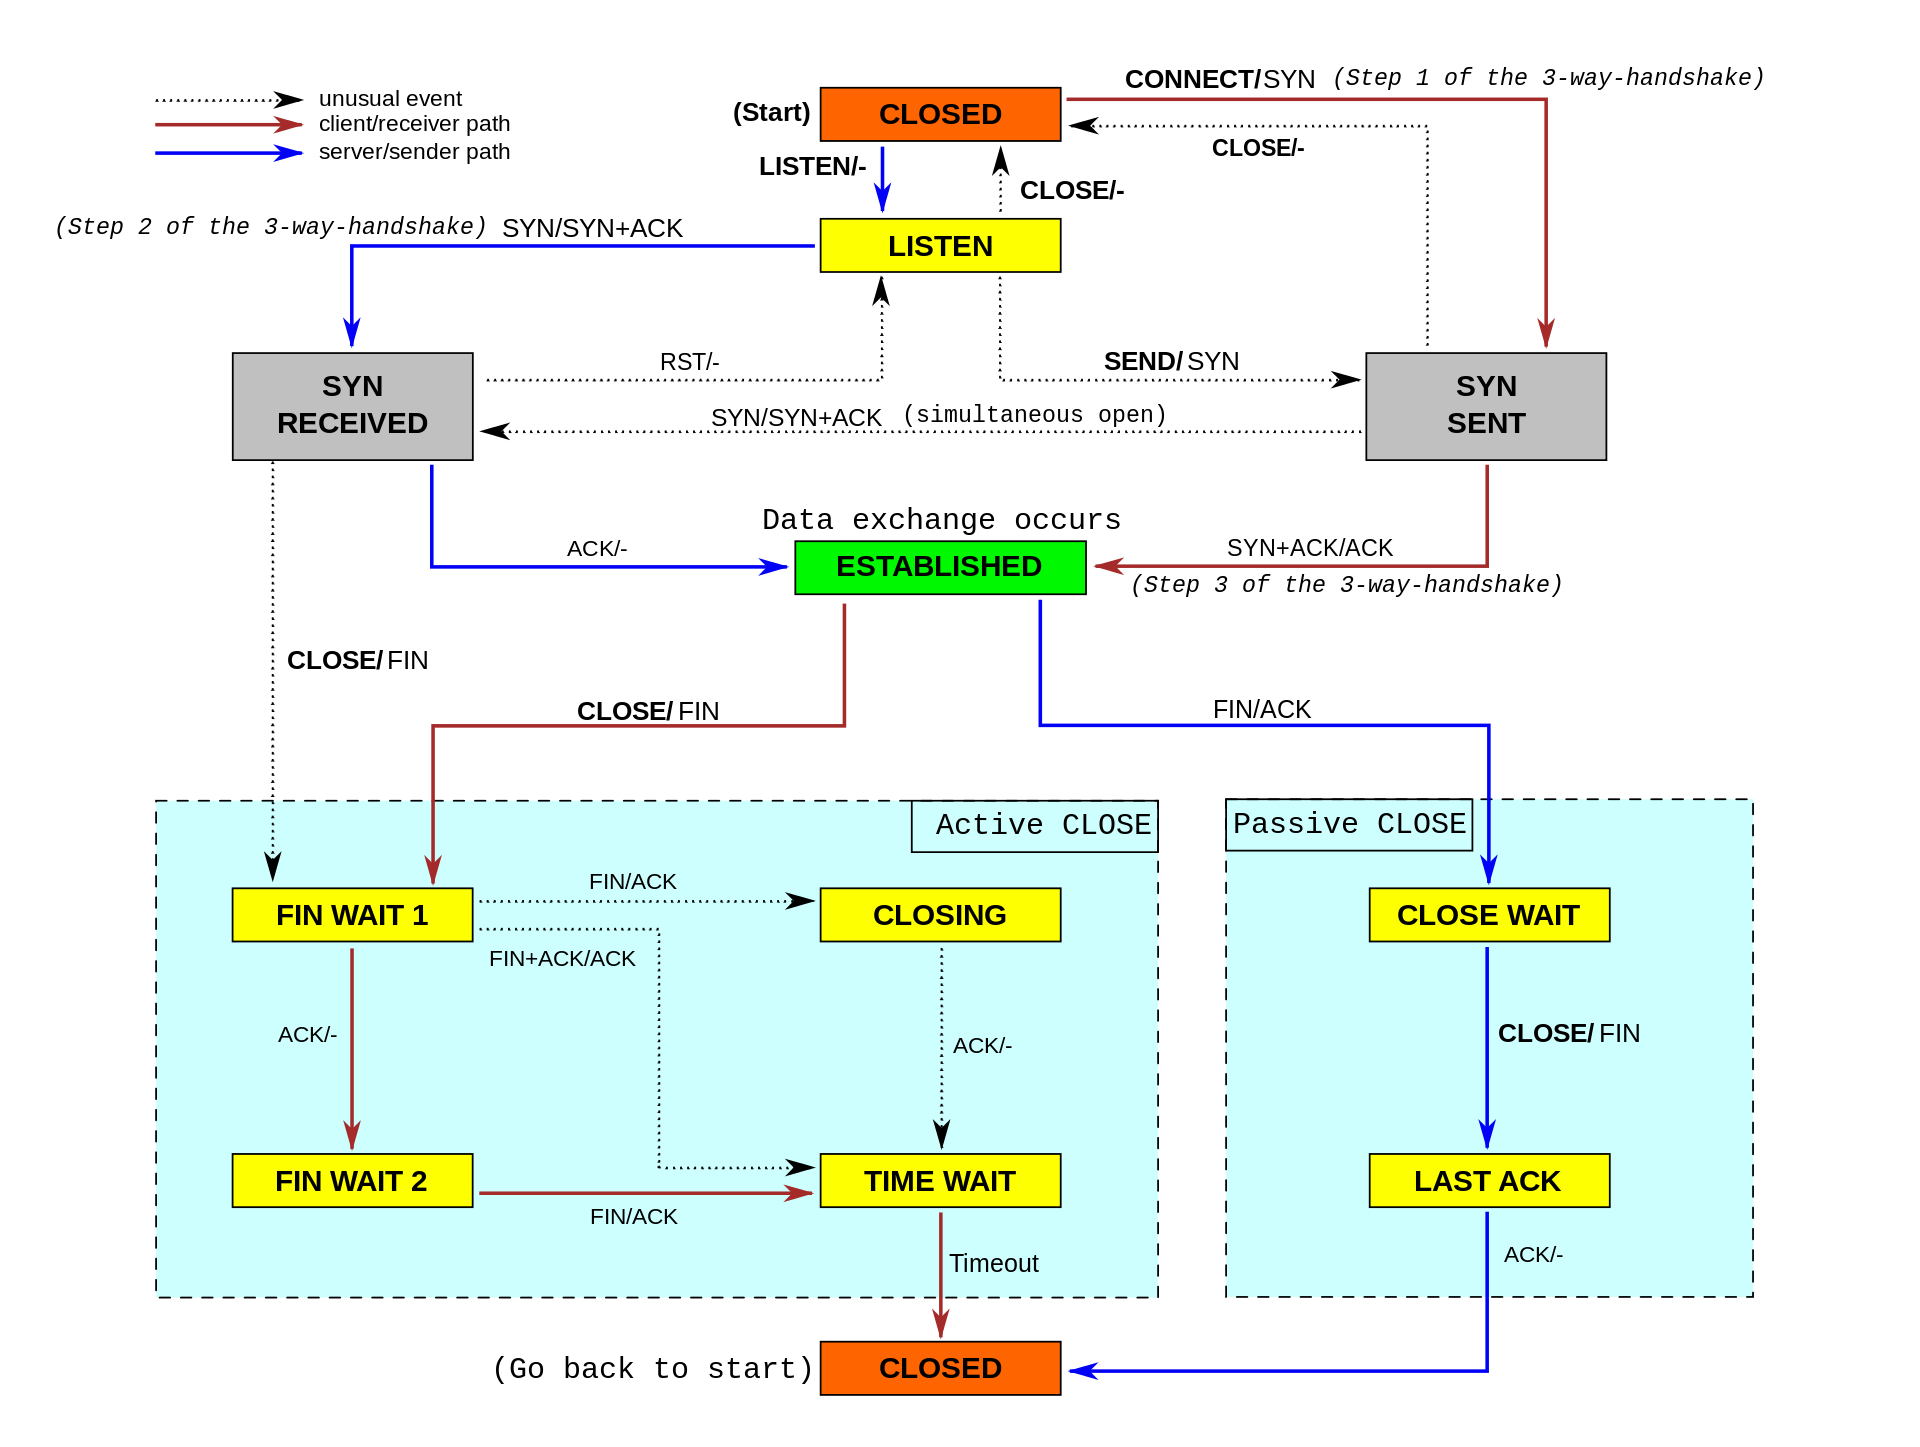
\includegraphics[width=\columnwidth]{../assets/Tcp-state-diagram-fixed-new.png}
  \caption{TCP State Diagram}
  % \label{fig:-assets-Tcp_state_diagram_fixed_new-svg-png}
  https://en.wikipedia.org/wiki/Transmission\_Control\_Protocol\#/media/File:Tcp\_state\_diagram\_fixed\_new.svg
\end{figure}

\section{Application Layer}
\begin{quotebox}
  An application layer is an abstraction layer that specifies the shared communications protocols and interface methods used by hosts in a communications network. An application layer abstraction is specified in both the Internet Protocol Suite (TCP/IP) and the OSI model. Although both models use the same term for their respective highest-level layer, the detailed definitions and purposes are different

  From: https://en.wikipedia.org/wiki/Application\_layer
\end{quotebox}
\subsection{DNS}
Domain Name Service is part of the application layer which goes on top of UDP or TCP. This protocol allows us the bind a name to another name, IP, or set of IPs.
{\centering
\begin{DndTable}[color=PhbLightGreen]{XX}
  \textbf{Type} & \textbf{What it represents} \\
  A & A record that point to an IPV4 address \\
  AAAA & A record that points to an IPV6 address \\
  CNAME & A record that points to another name \\
\end{DndTable}}
You can use programs like \texttt{host}, \texttt{dig}, or \texttt{nslookup} to check names.
Because a \texttt{CNAME} record points to another name and that name could be another \texttt{CNAME} record this DNS behaviour can be recursive until it reaches an IP address or a set of addresses.


\subsection{Firewalls}
Usually prevents hosts from communicating on certain ports, or hosting services like port ssh, ftp, etc.
HTTP and firewalls means that web clients are unlikely to be web servers as well. That communication must be initiated by clients rather then web services.


\section{Internet Protocol Stack}
Exchanging data over the internet uses multiple different standard and protocols that are built upon each other.

{\centering
\begin{DndTable}[color=PhbLightGreen]{XX}
  \textbf{Layer} & \textbf{Examples} \\
  Application & DNS, HTTP(S), SSL, SSH, etc \\
  Transport & TCP, UDP, etc \\
  Internet & IPV4/6, ICMP, etc \\
  Link & Ethernet, Wi-Fi, DSL, ARP, etc \\
\end{DndTable}}
Like layers of an onion each layer is wrapped inside each other.
The Application layer is wrapped inside the Transport layer which is wrapped inside an Internet layer which is finally wrapped inside a Link layer.
Which layers are used depends on the application, context, and physical medium used to communicate on the internet. 


\begin{Note}
  For HTTPS the TLS layers goes in between the TCP and HTTP layer. There is an additional handshake that is done so that both the client and server can encrypt and decrypt the data. 
  This add overhead as well as not encrypt anything below the transport layer. Meaning a sniffer can read the transport, internet and link layers. 
  Basically they can see who you are talking to.
\end{Note}
\newpage
\section{Review}
  \paragraph{Ethernet} 
  \begin{itemize}
    \item The lowest protocol on the network stack, everything is encompassed within it. It's one example of the Link Layer.
    \item It's old but we still use it. 
    \item Payload size is between 46 and 1500. Total max size including the header minus the preamble and delimiter is 1518. 
  \end{itemize}

  \paragraph{IPV4}
  \begin{itemize}
    \item The second lowest protocol on the network stack, encompassed within the Link Layer, it handles the routing and addressing between one computer and another. It's one example of the Internet Layer.
    \item We are running out of them due to the number of interconnected devices
    \item Header is pretty complicated with options and stuff.
    \item Max payload size is \(2^{16} = 65536\) bytes including all the headers and payloads above it or anything being encapsulated by it. But not including the IPV4 header itself.
  \end{itemize}

  \paragraph{IPV6}
  \begin{itemize}
    \item Like IPV4 it's the second lowest protocol on the network stack, encompassed within the Link Layer, it handles the routing and addressing between one computer and another. It's one example of the Internet Layer.
    \item We can more of these \(2^{128}\) a number with 39 digit or a big fucking number. 
    \item Header is a lot simpler as the task like checksuming is handled off to other layers like Link or Transport.
    \item Max payload size is \(2^{16} = 65536\) bytes including all the headers and payloads above it or anything being encapsulated by it. But including the IPV6 header itself.
  \end{itemize}
  
  \paragraph{UDP}
  \begin{itemize}
    \item Simple, connectionless protocol for the Transport Layer or the third layer in the network stack. 
    \item Used in DNS, and NTP queries for something simple or small. 
    \item Message packets are not guaranteed to be in order. 
    \item Max payload size is \(2^{16} = 65536\) bytes including everything the UDP packet/message is encapsulating. But not including the 8 bytes for the header.  
  \end{itemize}

  \paragraph{TCP}
  \begin{itemize}
    \item A more complicated, connection (or state) based protocol that is part of the Transport Layer like UDP. 
    \item Has a three way handshake to establish communication, using SYN, SYN+ACK, ACK.
    \item Active Close is client driven
    \item Passive Close is server driven
  \end{itemize}

  \paragraph{DNS}
  \begin{itemize}
    \item Domain Name Service, part of the Application Layer or the last (top) layer in the network stack.
    \item Used to resolve domain names to IP addresses
    \item Made up wih different records, A for IPV4, AAAA for IPV6, CNAME which points to another name
  \end{itemize}
\end{document}
